%!TEX program = xelatex
%========================================================================================================
% Workshop de Design Sprint e Material Design
%
% - Based on 'MaterialCv' (https://github.com/amng/MaterialCv)
% - To generate the poster, use xelatex.
% - It depends on the 'Roboto' fonts being installed, and on the
%   latex package 'euenc'
%
%========================================================================================================

\documentclass{article}
\usepackage[top=0cm, bottom=2cm, outer=0cm, inner=0cm]{geometry}
\usepackage[pages=some]{background}
\usepackage{xcolor}
\usepackage{fontspec}
\usepackage{multicol}


%Color definition based on Material Design
\definecolor{materialGreen} 	{RGB}{068,225,130}
\definecolor{materialGreenDark} {RGB}{029,184,090}
\definecolor{materialRed}   	{RGB}{218,068,049}
\definecolor{materialRedDark}   {RGB}{173,045,031}
\definecolor{materialPurple}   	{RGB}{153,039,176}
\definecolor{materialPurpleDark}{RGB}{088,022,099}
\definecolor{materialBlue}  	{RGB}{044,116,246}
\definecolor{materialBlueDark}  {RGB}{010,082,216}
\definecolor{materialYellow}	{RGB}{254,193,005}
\definecolor{materialYellowDark}{RGB}{194,147,001}
\definecolor{textGray}			{RGB}{070,070,070}
\definecolor{textLightGray}		{RGB}{140,140,140}

%Using font Roboto as main font for the document
\setmainfont{Roboto}

\backgroundsetup{
scale=1,
color=black,
opacity=0.6,
placement=top,
angle=0,
contents={%
  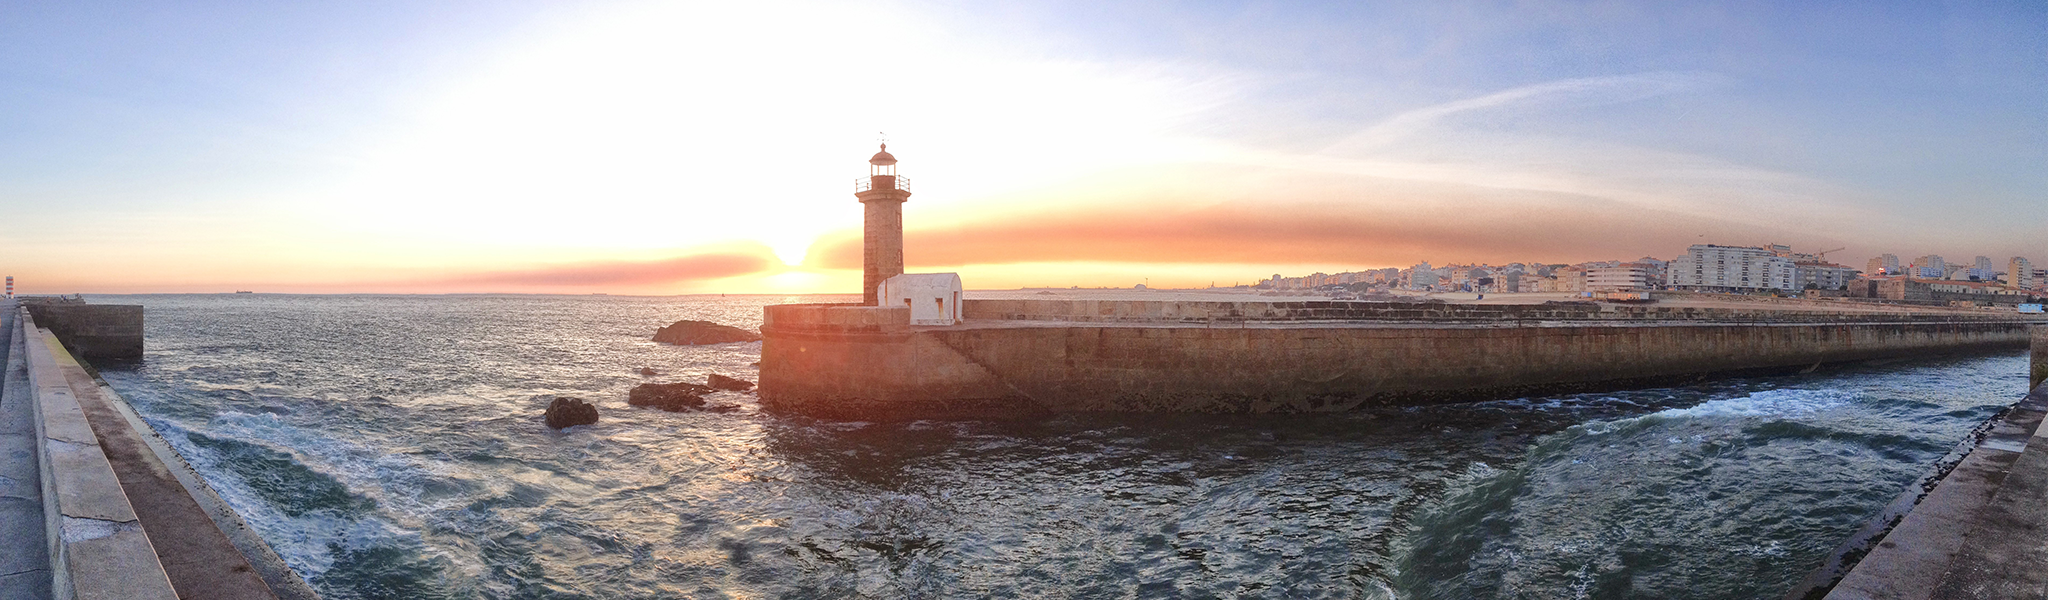
\includegraphics[width=\paperwidth,height=165pt]{"images/pic.jpg"}
  }%
}
\begin{document}
	\color{textGray}
	\pagenumbering{gobble}
	\vspace*{70pt} %spacing used to move the first and last name down
	\Huge
	\BgThispage
		\textcolor{black}{\textbf{Workshop de Design Sprint}}

		\textcolor{black}{\textbf{e Material Design}}
	\BgThispage
	\vspace*{20pt}

	% Inclui separadamente as seções do poster
	%!TEX root = cv.tex

% TODO: get the 'images/green/arrow75.png' in materialRed color.
%%Command used in order to make each entry cleaner
\newcommand{\QuestionEntry}[1]{
	$\begin{array}{l}
	{
\includegraphics[height=15pt]{images/green/arrow75red}}
	\end{array}
	$ #1
}

\LARGE
\noindent\colorbox{materialRed}
{\parbox[c][25pt][c]{\textwidth}{\hspace{15pt}\textcolor{white}{Por que participar?}}} %%Contacts separator

%%Contact Information
\large
\vspace*{10pt}
\QuestionEntry{Gosta de Software Livre?}

\QuestionEntry{Quer interagir com designers, programadores, artistas e com muitos outros especialistas?}

\QuestionEntry{Tem interesse em conhecer uma nova forma de estruturar, prototipar e validar ideias?}

\QuestionEntry{O que acha de aprender junto conosco a aplicar especificações de design?}


\vspace*{5pt}


	%!TEX root = cv.tex
\newcommand{\textBox}[1]{
\hspace*{7pt}
\begin{tabular}{  p{\dimexpr 0.97\linewidth-2\tabcolsep} }
  	{\normalsize #1}
\end{tabular}
\vspace*{10pt}
}

\newcommand{\designEntry}[2]{
	$\begin{array}{l}
	{\includegraphics[height=15pt]{#1}}
	\end{array}
	$ #2
}
\LARGE
\noindent\colorbox{materialYellow}
{\parbox[c][25pt][c]{\textwidth}{\hspace{15pt}\textcolor{white}{Design Sprint}}} %%Contacts separator

%%Contact Information
\large
\vspace*{10pt}

\textcolor{materialYellow}{Design Sprint} é um processo que busca
respostas rápidas para diversos tipos de problemas através de

\vspace*{10pt}

design, prototipagem, e testes com clientes; e é uma das metodologias da moda em
estratégias de

\vspace*{10pt}

negócios, inovação, ciência comportamental, design thinking,
e mais.

\vspace*{10pt}


	%!TEX root = cv.tex

% TODO: get the 'images/green/arrow75.png' in materialBlue color.
%%Command used in order to make each entry cleaner

\LARGE
\noindent\colorbox{materialBlue}
{\parbox[c][25pt][c]{\textwidth}{\hspace{15pt}\textcolor{white}{Material Design}}} %%Contacts separator

%%Contact Information
\large
\vspace*{10pt}

\textcolor{materialBlue}{Material Design} é uma especificação de design que visa
desenvolver um sistema básico que permita uma

\vspace*{10pt}

experiência unificada entre plataformas e tamanhos de
dispositivos.

\vspace*{10pt}


	%!TEX root = cv.tex

%%Command used in order to make each entry cleaner
\newcommand{\AwardEntry}[4]{
\begin{tabular}{ l l r }
  \textbf{\textcolor{materialPurple}{#1}}\hspace{20pt} & \textbf{#2} & {\small \textcolor{textLightGray}{#4}}\\
  	& \normalsize #3\\
\end{tabular}
\vspace*{10pt}
}

\LARGE
\noindent\colorbox{materialPurple}
{\parbox[c][25pt][c]{\textwidth}{\hspace{15pt}\textcolor{white}{Evento}}} %%Contacts separator

%%Contact Information
\large
\vspace*{10pt}

%Add new or alter education entries in this section by using the examples below
%\EducationEntry{starting year}{final year}{Type of studies}{Studies description if applicable}{Place of studies}

     Vamos juntos aplicar os princípios de       
     Design Sprint a desafios de usabilidade no   
	 software livre
	 
\vspace*{10pt}
	 Mezuro (\textcolor{materialPurple}{www.mezuro.org}) 
     desenvolvido no CCSL. Com os resultados      
     obtidos vamos então aprender como
	 
\vspace*{10pt}
	 traduzir  
     os protótipos finais em software funcional  
     utilizando os princípios de Material        
     Design.                                      

\vspace*{10pt}


	%!TEX root = cv.tex

\newcommand{\ContactEntry}[2]{
	$\begin{array}{l}
	{\includegraphics[height=18pt]{#1}}
	\end{array}
	$ #2
}


\LARGE
\noindent\colorbox{materialGreen}
{\parbox[c][25pt][c]{\textwidth}{\hspace{15pt}\textcolor{white}{Contato}}} %%Contacts separator

\begin{multicols}{3}

%%Contact Information
\large
%Add new or alter contact entries in this section by using the examples below
%for other contact information search the image folder for other icons

\ContactEntry{images/green/mail9}{mezurometrics@gmail.com}

\ContactEntry{images/green/black70}{17 de novembro - 8h às 14h

\hspace*{28pt} 18 de novembro - 13h às 18h
}

\columnbreak

\ContactEntry{images/green/house3}{Auditório do CCSL

\hspace*{28pt} IME - USP

\hspace*{28pt} Rua do Matão, 1010}

\columnbreak

\hspace*{25pt} Inscreva-se
\vspace{.5cm}

\hspace*{25pt} 
\includegraphics[height=90pt]{images/design_sprint_form_qr.png}

\end{multicols}

\end{document}
